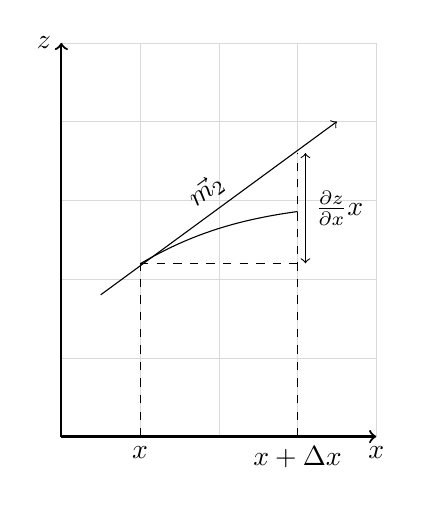
\begin{tikzpicture}
  \draw[very thin, gray!30, step = 1cm] (0, 0) grid (4, 5);
  \draw[domain = 1 : 3, variable = \x]
    plot ({\x}, {3 / (1 + e^(-\x))});

  \draw[thick] [->] (0, 0) -- (4, 0) node[right, below] {\(x\)};
  \draw[thick] [->] (0, 0) -- (0, 5) node[above, left] {\(z\)};

  \draw node[below] at (1, 0) {\(x\)};
  \draw node[below] at (3, 0) {\(x + \Delta x\)};

  \draw[dashed] (1, 0) -- (1, 2.2);
  \draw[dashed] (3, 0) -- (3, 3.6);

  \draw[dashed] (1, 2.2) -- (3, 2.2);
  \draw[<->] (3.1, 2.2) -- (3.1, 3.6)
    node[midway, right] {\(\frac{\partial z}{\partial x} \dd x\)};

  \draw[->] (0.5, 1.8) -- (3.5, 4)
    node[midway, above, sloped] {\(\vec{m_{2}}\)};
\end{tikzpicture}
